\documentclass[a4paper,11pt,fleqn]{article}%fleqn pour aligner les equations à gauche

\usepackage{../../Styles/Eval}

\newcommand{\chnum}{Chapitre 12}
\newcommand{\chtitle}{Mouvements dans un champ uniforme}
\newcommand{\dtype}{Eval}

\begin{document}
	\maketitle
\section{Le Mölkky}
Le Mölkky, créé en 1996, est un jeu de plein air orifinaire de Finlande.
Dans ce jeu, le joueur doit faire tomber des quilles en bois, à l'aide d'un bâton, afin d'atteindre un score de 50 points.\\
Une quille tombée lui donnera le nombre de points dur cette dernière, compris entre 1 et 12. Plusieurs quilles tombées donneront au joueur le nombre de points correspondant au nombre de quilles au sol.\\

L'objectif de cet exercice est d'établir l'équation horaire de la trajectoire du bâton lancé et de déterminer le lieu d'impact au sol afin de prévoir une éventuelle vuctoire d'un joueur.

\begin{figure}[h!]
\begin{minipage}{.6\linewidth}
    On s'intéresse au mouvement du centre de masse $G$ du bâton lorsqu'un joueur le lance afin de faire tomber une quille. L'étude est réalisée dans le référentiel terrestre supposé galiléen et on considère qu'une fois lancé, le bêton n'est soumis qu'ç son poids. Pour simplifier, on suppose que le bâton ne tourne pas sur lui-même. La masse du bâton est notée $m$.\\
    Quand le bêton quitte la main du joueur, son centre de masse $G$ est situé à une heuteur $h$ par rapport au sol avec un vecteur vitesse initiale $\vv{v_0}$ qui forme un angle $\alpha$ avec l'horizontale.\\
    On étudie le mouvement du centre de masse du système {bâton} dans le repère cartésien indique sur le Doc.~\ref{doc1}    
\end{minipage}
\begin{minipage}{.38\linewidth}
    \caption{Schémam de la situation du lancer}
    \label{doc1}
    \centering
    \begin{tikzpicture}
        \draw[-Latex] (0,0) -- (4,0);
        \draw[-Latex] (0,0) -- (0,4.5);
        \draw[dashed] (0,2.5) -- (4,2.5);
        \draw[-Latex] (0,2.5) -- (2,4);
        \draw[Latex-Latex,dashed] (3,0) -- (3,2.5);
        \draw[-Latex,thick] (0,0)--(1,0);
        \draw[-Latex,thick] (0,0)--(0,1);


        \node[below] (i) at (.5,0){$\vv{i}$};
        \node[below left] (x) at (4,0){$x$};
        \node[below left] (O) at (0,0){$O$};

        \node[left] (j) at (0,.5){$\vv{j}$};
        \node[left] (y) at (0,4){$y$};

        \node[left] (G) at (0,2.5){$G(0)$};

        \node[right] (alpha) at (1.5,3){$\alpha$};

        \node[right] (v0) at (2,4){$\vv{v_0}$};
    \end{tikzpicture}
\end{minipage}
\end{figure}

\begin{enumerate}
    \item Énoncer la deuxième loi de Newton et l'utiliser pour établir les expressions des coordonnées notées $a_x(t)$ et $a_y(t)$ du vecteur accélération $\vv{a(t)}$ du point $G$ selon les axes ($Ox$) et ($Oy$).
    \item Établir les expressions des coordonnées horizontales notées $v_x(t)$ et verticales $v_y(t)$ du vecteur vitesse $\vv{v(t)}$ du point $G$.
    \item À partir des expressions des coordonnées de la vitesse $v_x(t)$ et $v_y(t)$ et du Doc.~\ref{doc1}, établir que les équations horaires du mouvement $x(t)$ et $y(t)$ du point $G$ sont : 
    \[
        \left\{
        \begin{array}{l}
        x(t) = v_0 \cdot \cos(\alpha) \cdot t \\[4pt]
        y(t) = - \dfrac{1}{2} g \cdot t^2 + v_0 \cdot \sin(\alpha)\cdot t + h
        \end{array}
        \right.
    \]
\end{enumerate}

\begin{data}
    \begin{itemize}
        \item vitesse initiale de lancer du bâton de Mölkky : $v_0 = \SI{4,9}{\meter\per\second}$
        \item hauteur depuis laquelle le bâton est lancé : $h = \SI{.70}{\meter}$
        \item angle avec lequel le bâton est lancé par rapport à l'horizontale : $\alpha = \SI{30}{\degree}$
        \item intensité du champ de pesanteur terrestre : $g = \SI{9.8}{\meter\per\second}$
    \end{itemize}
\end{data}

\begin{enumerate}[resume]
    \item À l'aide des données et des équations horaires du mouvement, montrer que l'expression de l'équation de la trajectoire $y(x)$, $x$ et $y$ étant exprimés en mètres, s'écrit dous la forme : $$y(x) = -0.27 x^2 + 0,58 x + 0,70$$
\end{enumerate}
Un joueur ayant déjà marqué 41 points s'apprête à lancer le bâton de Mölkky. Pour gagner, il doit atteindre exactement le score de 50 points. La configuration du jeu est représentée sur la photographie du doc.~\ref{doc2}.

\begin{figure}[h!]
    \caption{Photographie de la configuration du jeu avant le lancer}
    \label{doc2}
    \centering
    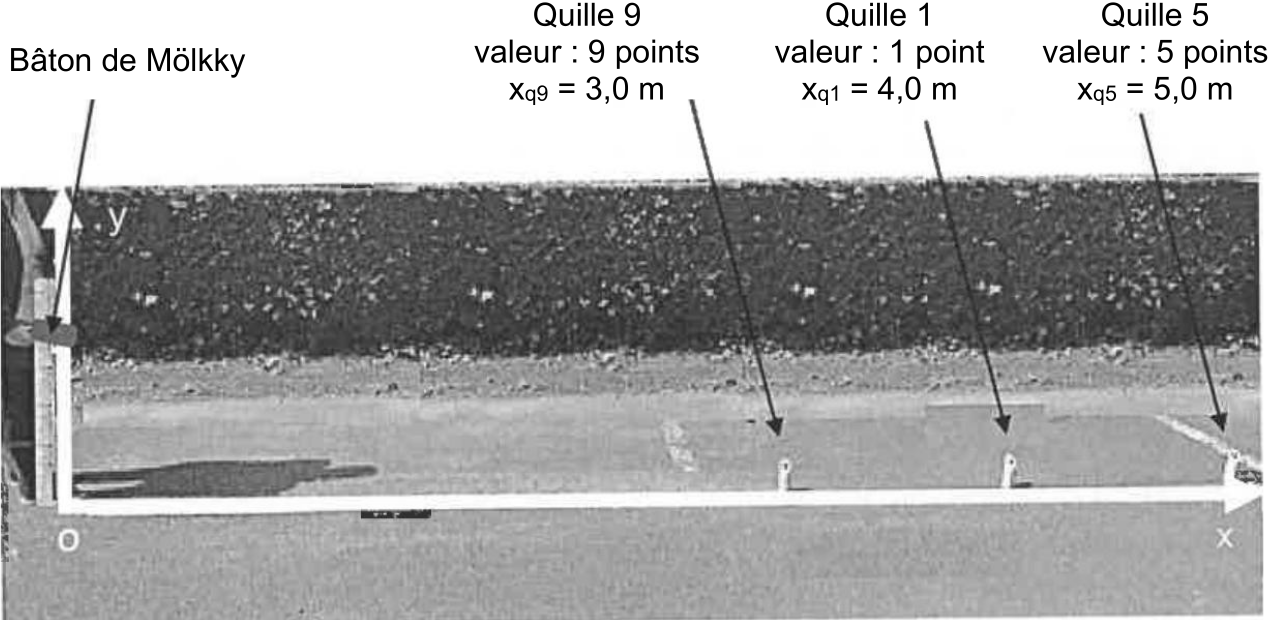
\includegraphics[width=\linewidth]{Ressources/TSPE_DS2_25_Fig2.png}
\end{figure}

Dans notre étude, la taille des quilles est considérée comme négligeable au regard des distances mises en jau. On assimilera alors la quille à un point posé au sol. On suppose qu'il n'y a pas de rebond du bâton à la suite du lancer.\\
\textit{Dans la question suivante, le candidat est invité à prendre des initiatives et à présenter la démarche quivie, même si elle n'a pas abouti. La démarche est évaluée et nécessite d'être correctement présentée.}

\begin{enumerate}[resume]
    \item Vérifier que la partie est remportée par le joueur si le lancer est réalisé dans les conditions précisées dans les données précédentes.
\end{enumerate}

Sur le doc.~\ref{doc3}, on a reproduit un extrait d'un programme Python qui permet de calculer puis de tracer les courbes représentant l'énergie cinétique $E_c$, l'énergie potentielle de pesanteur $E_p$ et l'énergie mécanique $E_m$ du bâton de Mölkky lors de son lancer. Les données numériques utilisées sont identiques aux questions présécentes.

\begin{figure}[h!]
    \caption{Extrait du programme python}
    \label{doc3}
    \begin{lstlisting}[language=Python]
# [...] lignes precedentes

Ecl = []
Epl = []
Eml = []

for i in range(len(tl)):
    Ec = 0.5 * 0.4 * (vxl[i]**2 + vyl[i]**2)
    Ecl.append(Ec)

    Ep = 0.4 * 9.81 * y[i]
    Epl.append(Ep)

    Em = 
    Eml.append(Em)

# [...] lignes suivantes
\end{lstlisting}
\end{figure}

\begin{enumerate}[resume]
    \item À partir du doc.~\ref{doc3}, déterminer la masse $m$ du bâton de Mölkky. justifier la réponse.
    \item Écrire et compléter, sur votre copie, la ligne 15 du programme du doc.~\ref{doc3} qui permet de calculer l'énergie mécanique $E_m$ du bâton de Mölkky.
\end{enumerate}
Le doc.~\ref{doc4} représente les courbes affichées après avoir exécuté le programme Python complet.
\begin{figure}[h!]
    \caption{Évolution temporelle des énergies}
    \label{doc4}
    \centering
    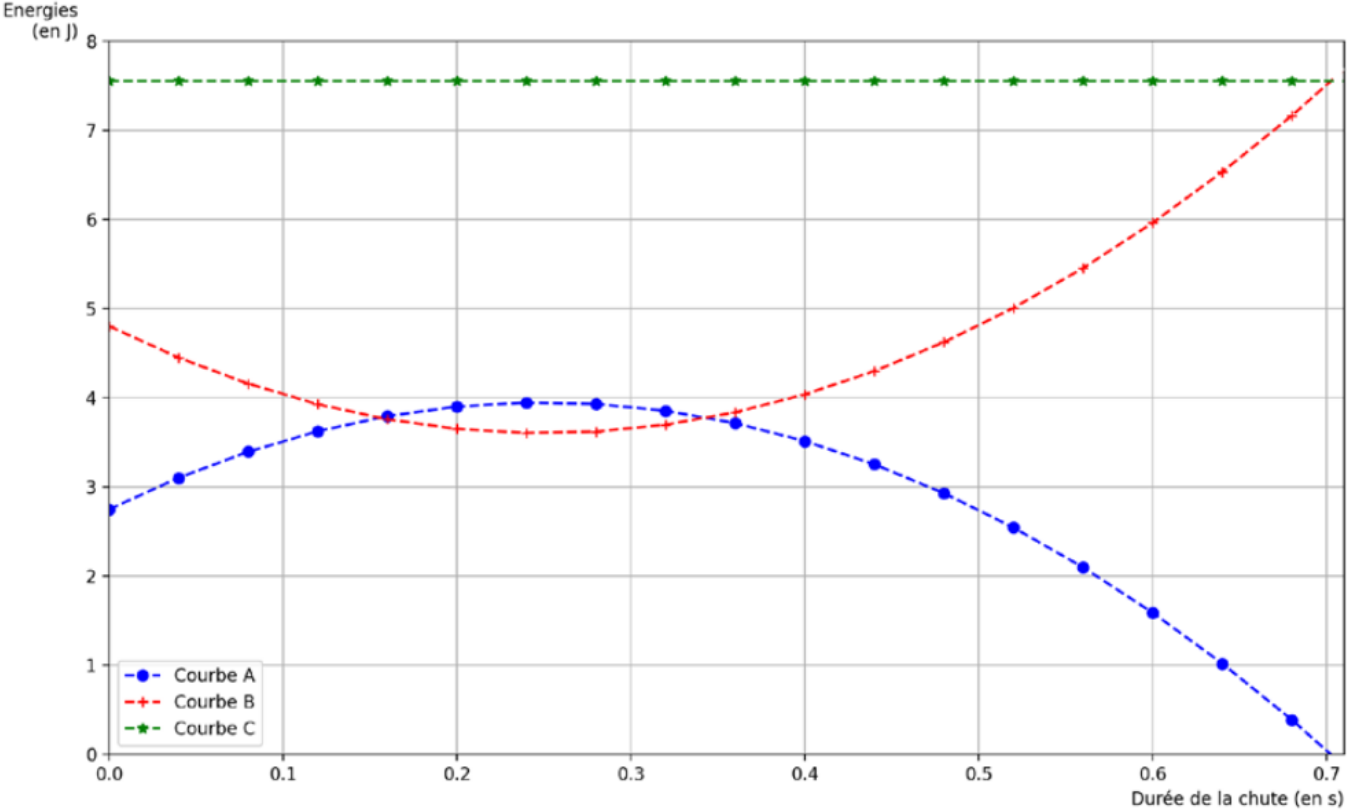
\includegraphics[width = .6\linewidth]{Ressources/TSPE_DS2_25_Fig4.png}
\end{figure}

\begin{enumerate}[resume]
    \item Attribuer chaque courbe du doc.~\ref{doc4} à l'énergie représentée. Justifier la réponse.
    \item Déterminer la "durée de vol" du bêton de Mölkky (durée de chute) et en déduire que la partie décrite précédemment est remportée par le joueur, en considérant les équations horaires du mouvement établies dans la question 3.
\end{enumerate}

\section{Le scanner à rayons X}
La radiographie réalisée par un scanner à rayons X est une technique d'imagerie médicale utile dans le diagnostique de nombreuses pathologies.\\
Le scanner crée un saisceau à rayons X à l'aide d'un tube à rayons X ou de Coolidge.
\begin{figure}[h!]
    \centering
    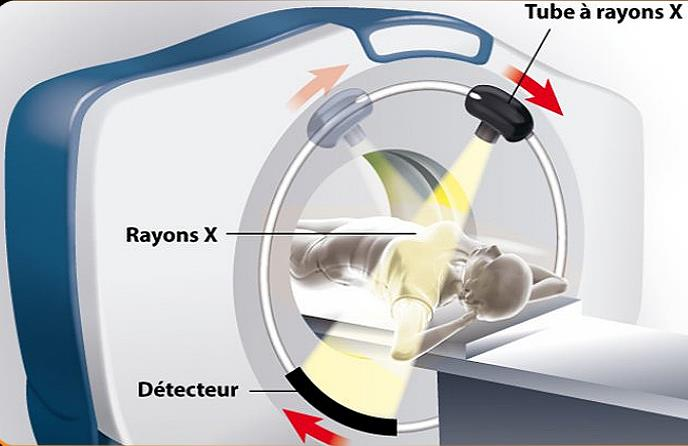
\includegraphics[width = .5\linewidth]{Ressources/TSPE_DS2_25_Fig5.png}
\end{figure}
Dans ce tube à rayons X, une tension élevée $U$ est maintenue entre un filament cathodique. borne négative, et une anode tournante, norne positive (doc.~\ref{doc5} et~\ref{doc6}). Un courant électrique provoque l'échauffement d'un filament situé à la cathode. L'agitation des électrons présents augente et une partie d'entre eux est éjectée du filament au point $O$, avec une vitesse négligeable. La tension $U$ accélère les électrons du point $O$ vers l'anode en tungstène. Denevus très énergétiques, ils frappent l'anode, ce qui produit des rayons X. Pour obtenir ces rayons X, chaque électron doit avoir acquis une énergie cinétique égale à \SI{6,4E-15}{J} au minimum.

\begin{figure}[h!]
    \begin{minipage}{.49\linewidth}
       \caption{Schéma du tube à rayons X}
       \label{doc5}
       \centering
       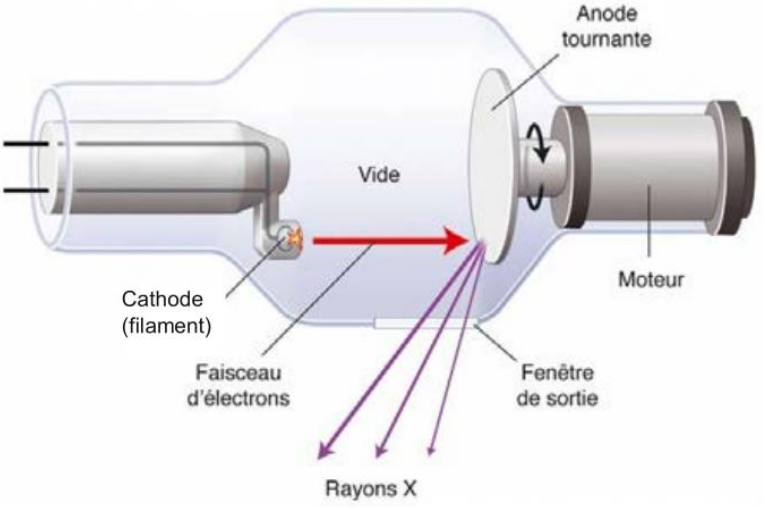
\includegraphics[width=.8\linewidth]{Ressources/TSPE_DS2_25_Fig6.png} 
    \end{minipage}
    \begin{minipage}{.49\linewidth}
       \caption{Schéma simplifié}
       \label{doc6}
       \centering
       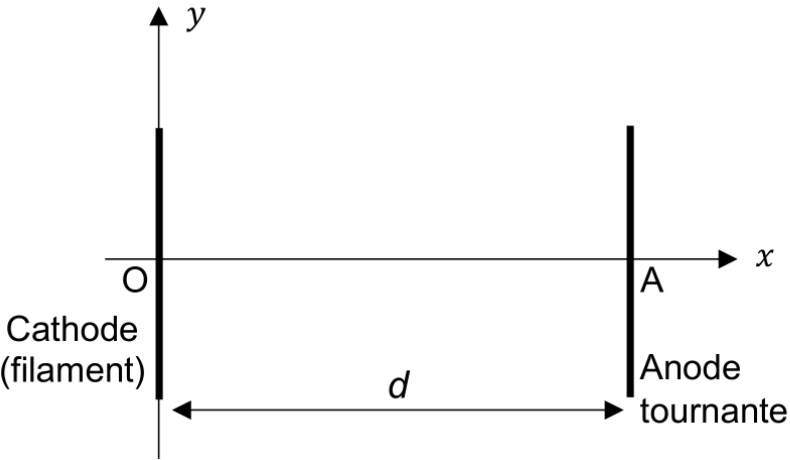
\includegraphics[width=.8\linewidth]{Ressources/TSPE_DS2_25_Fig7.png} 
    \end{minipage}
\end{figure}

Le but de cet exercice est de calculer la tension à appliquer entre la cathode et l'anode pour que le faisceau d'électrons parvienne à provoquer l'émission de photons X au niveau de l'anode. On considèrera l'électrons comme système d'étude assimilé à un point matériel dont on négligera le poids. Son mouvement sera étudié dans le référentiel terrestre considéré comme galiléen. on mouvement sera étudié dans un référentiel terrestre considéré comme galiléen. À l'instant initial, l'électron est situé au point $O$ et sa vitesse est considérée comme nulle.\\

\begin{data}
    \begin{itemize}
        \item Masse de l'électron : $m = \SI{9,1E31}{kg}$
        \item Charge de l'électrons : $q = -e = \SI{-1,6E-19}{C}$
    \end{itemize}
\end{data}

\begin{enumerate}
    \item Reproduire le doc.~\ref{doc5} puis tracer, entre la cathode et l'anode, sans préciser d'échelle :\begin{itemize}
        \item le vecteur champ électrique supposé uniforme $\vv{E}$
        \item la force $\vv{F}$ que subit un électron situé en un point de l'axe ($0x$)
    \end{itemize}
    \item Donner l'expression vectorielle de $\vv{F}$ en fonction de $e$ et $\vv{E}$.
    \item Montrer que les coordonnées du vecteur accélération $\vv{a}$ de l'électron, exprimées dans le repère ($Oxy$) du doc.~\ref{doc5}, sont $a_x = \dfrac{e\cdot U}{m \cdot d}$ et $a_y = 0$.
    \item En déduire le coordonnées du vecteur vitesse de l'électron selon l'axe ($Ox$), notée $v_x$. Établir que $x$ d'écrit $ \dfrac{1}{2} \cdot \left(\dfrac{e\cdot U}{m \cdot d}\right) \cdot t^2$.
    \item Donner l'expression litterale de $T_A$, l'instant où l'électron atteint l'anode (au point $A$) située à la distance $d$ de $O$
    \item Grâce aux deux questions précédentes, en déduire que l'expression de la vitesse de l'électron au niveau de l'anode est $v_A = \sqrt{\dfrac{2\cdot e \cdot U}{m}}$.
    \item Répondre à la problématique de l’exercice "trouver la tension minimale à appliquer entre la cathode et l’anode pour que le faisceau d’électron parvienne à provoquer l’émission de photons X an niveau de l’anode".
\end{enumerate}
\end{document}
